\documentclass[11pt,ignorenonframetext,]{beamer}
\setbeamertemplate{caption}[numbered]
\setbeamertemplate{caption label separator}{: }
\setbeamercolor{caption name}{fg=normal text.fg}
\beamertemplatenavigationsymbolsempty
\usepackage{lmodern}
\usepackage{amssymb,amsmath}
\usepackage{ifxetex,ifluatex}
\usepackage{fixltx2e} % provides \textsubscript
\ifnum 0\ifxetex 1\fi\ifluatex 1\fi=0 % if pdftex
  \usepackage[T1]{fontenc}
  \usepackage[utf8]{inputenc}
\else % if luatex or xelatex
  \ifxetex
    \usepackage{mathspec}
  \else
    \usepackage{fontspec}
  \fi
  \defaultfontfeatures{Ligatures=TeX,Scale=MatchLowercase}
\fi
\usetheme[]{metropolis}
% use upquote if available, for straight quotes in verbatim environments
\IfFileExists{upquote.sty}{\usepackage{upquote}}{}
% use microtype if available
\IfFileExists{microtype.sty}{%
\usepackage{microtype}
\UseMicrotypeSet[protrusion]{basicmath} % disable protrusion for tt fonts
}{}
\newif\ifbibliography
\hypersetup{
            pdftitle={Lecture 15},
            pdfauthor={Colin Rundel},
            pdfborder={0 0 0},
            breaklinks=true}
\urlstyle{same}  % don't use monospace font for urls
\usepackage{color}
\usepackage{fancyvrb}
\newcommand{\VerbBar}{|}
\newcommand{\VERB}{\Verb[commandchars=\\\{\}]}
\DefineVerbatimEnvironment{Highlighting}{Verbatim}{commandchars=\\\{\}}
% Add ',fontsize=\small' for more characters per line
\newenvironment{Shaded}{}{}
\newcommand{\KeywordTok}[1]{\textcolor[rgb]{0.00,0.44,0.13}{\textbf{#1}}}
\newcommand{\DataTypeTok}[1]{\textcolor[rgb]{0.56,0.13,0.00}{#1}}
\newcommand{\DecValTok}[1]{\textcolor[rgb]{0.25,0.63,0.44}{#1}}
\newcommand{\BaseNTok}[1]{\textcolor[rgb]{0.25,0.63,0.44}{#1}}
\newcommand{\FloatTok}[1]{\textcolor[rgb]{0.25,0.63,0.44}{#1}}
\newcommand{\ConstantTok}[1]{\textcolor[rgb]{0.53,0.00,0.00}{#1}}
\newcommand{\CharTok}[1]{\textcolor[rgb]{0.25,0.44,0.63}{#1}}
\newcommand{\SpecialCharTok}[1]{\textcolor[rgb]{0.25,0.44,0.63}{#1}}
\newcommand{\StringTok}[1]{\textcolor[rgb]{0.25,0.44,0.63}{#1}}
\newcommand{\VerbatimStringTok}[1]{\textcolor[rgb]{0.25,0.44,0.63}{#1}}
\newcommand{\SpecialStringTok}[1]{\textcolor[rgb]{0.73,0.40,0.53}{#1}}
\newcommand{\ImportTok}[1]{#1}
\newcommand{\CommentTok}[1]{\textcolor[rgb]{0.38,0.63,0.69}{\textit{#1}}}
\newcommand{\DocumentationTok}[1]{\textcolor[rgb]{0.73,0.13,0.13}{\textit{#1}}}
\newcommand{\AnnotationTok}[1]{\textcolor[rgb]{0.38,0.63,0.69}{\textbf{\textit{#1}}}}
\newcommand{\CommentVarTok}[1]{\textcolor[rgb]{0.38,0.63,0.69}{\textbf{\textit{#1}}}}
\newcommand{\OtherTok}[1]{\textcolor[rgb]{0.00,0.44,0.13}{#1}}
\newcommand{\FunctionTok}[1]{\textcolor[rgb]{0.02,0.16,0.49}{#1}}
\newcommand{\VariableTok}[1]{\textcolor[rgb]{0.10,0.09,0.49}{#1}}
\newcommand{\ControlFlowTok}[1]{\textcolor[rgb]{0.00,0.44,0.13}{\textbf{#1}}}
\newcommand{\OperatorTok}[1]{\textcolor[rgb]{0.40,0.40,0.40}{#1}}
\newcommand{\BuiltInTok}[1]{#1}
\newcommand{\ExtensionTok}[1]{#1}
\newcommand{\PreprocessorTok}[1]{\textcolor[rgb]{0.74,0.48,0.00}{#1}}
\newcommand{\AttributeTok}[1]{\textcolor[rgb]{0.49,0.56,0.16}{#1}}
\newcommand{\RegionMarkerTok}[1]{#1}
\newcommand{\InformationTok}[1]{\textcolor[rgb]{0.38,0.63,0.69}{\textbf{\textit{#1}}}}
\newcommand{\WarningTok}[1]{\textcolor[rgb]{0.38,0.63,0.69}{\textbf{\textit{#1}}}}
\newcommand{\AlertTok}[1]{\textcolor[rgb]{1.00,0.00,0.00}{\textbf{#1}}}
\newcommand{\ErrorTok}[1]{\textcolor[rgb]{1.00,0.00,0.00}{\textbf{#1}}}
\newcommand{\NormalTok}[1]{#1}
\usepackage{longtable,booktabs}
\usepackage{caption}
% These lines are needed to make table captions work with longtable:
\makeatletter
\def\fnum@table{\tablename~\thetable}
\makeatother
\usepackage{graphicx,grffile}
\makeatletter
\def\maxwidth{\ifdim\Gin@nat@width>\linewidth\linewidth\else\Gin@nat@width\fi}
\def\maxheight{\ifdim\Gin@nat@height>\textheight0.8\textheight\else\Gin@nat@height\fi}
\makeatother
% Scale images if necessary, so that they will not overflow the page
% margins by default, and it is still possible to overwrite the defaults
% using explicit options in \includegraphics[width, height, ...]{}
\setkeys{Gin}{width=\maxwidth,height=\maxheight,keepaspectratio}

% Prevent slide breaks in the middle of a paragraph:
\widowpenalties 1 10000
\raggedbottom

\AtBeginPart{
  \let\insertpartnumber\relax
  \let\partname\relax
  \frame{\partpage}
}
\AtBeginSection{
  \ifbibliography
  \else
    \let\insertsectionnumber\relax
    \let\sectionname\relax
    \frame{\sectionpage}
  \fi
}
\AtBeginSubsection{
  \let\insertsubsectionnumber\relax
  \let\subsectionname\relax
  \frame{\subsectionpage}
}

\setlength{\parindent}{0pt}
\setlength{\parskip}{6pt plus 2pt minus 1pt}
\setlength{\emergencystretch}{3em}  % prevent overfull lines
\providecommand{\tightlist}{%
  \setlength{\itemsep}{0pt}\setlength{\parskip}{0pt}}
\setcounter{secnumdepth}{0}

\usepackage{geometry}
\usepackage{graphicx}
\usepackage{amssymb}
\usepackage{color}          	% gives color options
\usepackage{url}		% produces hyperlinks
\usepackage[english]{babel}
\usepackage{colortbl}	% allows for color usage in tables
\usepackage{multirow}	% allows for rows that span multiple rows in tables
\usepackage{xcolor}		% this package has a variety of color options
\usepackage{calc}
\usepackage{multicol}
\usepackage{wrapfig}
\usepackage{textcomp}
\usepackage{bm}
\usepackage{bbm}
\usepackage{setspace}
\usepackage{changepage}
\singlespacing

%%%%%%%%%%%%%%%%
% Small code output
%%%%%%%%%%%%%%%%

%% change fontsize of R code

\makeatletter
\@ifundefined{Shaded}{\newenvironment{Shaded}{}{}}{}
\makeatother


\let\oldShaded\Shaded
\let\endoldShaded\endShaded
\renewenvironment{Shaded}{\footnotesize\begin{spacing}{0.9}\oldShaded}{\endoldShaded\end{spacing}}

%% change fontsize of output
\let\oldverbatim\verbatim
\let\endoldverbatim\endverbatim
\renewenvironment{verbatim}{\footnotesize\begin{spacing}{0.9}\oldverbatim}{\endoldverbatim\end{spacing}}


\newcommand{\tinyoutput}{
  \renewenvironment{Shaded}{\tiny\begin{spacing}{0.9}\oldShaded}{\endoldShaded\end{spacing}}
  \renewenvironment{verbatim}{\tiny\begin{spacing}{0.9}\oldverbatim}{\endoldverbatim\end{spacing}}
}

\newcommand{\scriptoutput}{
  \renewenvironment{Shaded}{\scriptsize\begin{spacing}{0.9}\oldShaded}{\endoldShaded\end{spacing}}
  \renewenvironment{verbatim}{\scriptsize\begin{spacing}{0.9}\oldverbatim}{\endoldverbatim\end{spacing}}
}

\newcommand{\footnoteoutput}{
  \renewenvironment{Shaded}{\footnotesize\begin{spacing}{0.9}\oldShaded}{\endoldShaded\end{spacing}}
  \renewenvironment{verbatim}{\footnotesize\begin{spacing}{0.9}\oldverbatim}{\endoldverbatim\end{spacing}}
}

%\newcommand{\verbatimfont}[1]{\renewcommand{\verbatim@font}{\ttfamily#1}}


%%%%%%%%%%%%%%%%
% Custom Colors
%%%%%%%%%%%%%%%%

\xdefinecolor{oiBlue}{rgb}{0.15, 0.35, 0.55}
\xdefinecolor{gray}{rgb}{0.5, 0.5, 0.5}
\xdefinecolor{darkGray}{rgb}{0.3, 0.3, 0.3}
\xdefinecolor{darkerGray}{rgb}{0.2, 0.2, 0.2}
\xdefinecolor{rubineRed}{rgb}{0.89,0,0.30}
\xdefinecolor{linkCol}{rgb}{0.11,0.49,0.95}	
\xdefinecolor{irishGreen}{rgb}{0,0.60,0}	
\xdefinecolor{darkturquoise}{rgb}{0.44, 0.58, 0.86}
\definecolor{lightGreen}{rgb}{0.533,0.765,0.42}
%\xdefinecolor{hlblue}{rgb}{0.051,0.65,1}
\xdefinecolor{hlblue}{rgb}{ 0.055, 0.639, 0.831}
\definecolor{light}{rgb}{.337,.608,.741}
\definecolor{dark}{rgb}{.337,.608,.741}

\definecolor{cpink}{rgb}{0.93, 0.23, 0.51}

%%%%%%%%%%%%%%%%
% Custom Commands
%%%%%%%%%%%%%%%%

% text colors
\newcommand{\red}[1]{\textit{\textcolor{rubineRed}{#1}}}
\newcommand{\orange}[1]{\textit{\textcolor{orange}{#1}}}
\newcommand{\pink}[1]{\textit{\textcolor{rubineRed!90!white!50}{#1}}}
\newcommand{\green}[1]{\textit{\textcolor{irishGreen}{#1}}}
\newcommand{\blue}[1]{\textit{\textcolor{darkturquoise}{#1}}}
\newcommand{\light}[1]{\textcolor{light}{\textbf{#1}}}
\newcommand{\dark}[1]{\textcolor{dark}{#1}}
\newcommand{\gray}[1]{\textcolor{gray}{#1}}


% links: webURL, webLin, appLink
\newcommand{\webURL}[1]{\urlstyle{same}{\textit{\textcolor{linkCol}{\url{#1}}} }}
\newcommand{\webLink}[2]{\href{#1}{\textcolor{linkCol}{{#2}}}}
\newcommand{\appLink}[2]{\href{#1}{\textcolor{lightGreen!80!black!90}{{#2}}}}

% mail
\newcommand{\mail}[1]{\href{mailto:#1}{\textit{\textcolor{linkCol}{#1}}}}

% highlighting: hl, hlGr, mathhl
\newcommand{\hl}[1]{\textit{\textcolor{hlblue}{#1}}}
\newcommand{\hlGr}[1]{\textit{\textcolor{lightGreen}{#1}}}
\newcommand{\hlRd}[1]{\textit{\textcolor{rubineRed}{#1}}}
\newcommand{\mathhl}[1]{\textcolor{hlblue}{\ensuremath{#1}}}

% example
\newcommand{\ex}[1]{\textcolor{blue}{{{\small (#1)}}}}


\DeclareMathOperator*{\argmin}{arg\,min}
\DeclareMathOperator*{\argmax}{arg\,max}

\title{Lecture 15}
\subtitle{Mauna Loa Example \& GPs for GLMs}
\author{Colin Rundel}
\date{03/08/2017}

\begin{document}
\frame{\titlepage}

\section{Mauna Loa Exampel}\label{mauna-loa-exampel}

\begin{frame}{Atmospheric CO\(_2\)}

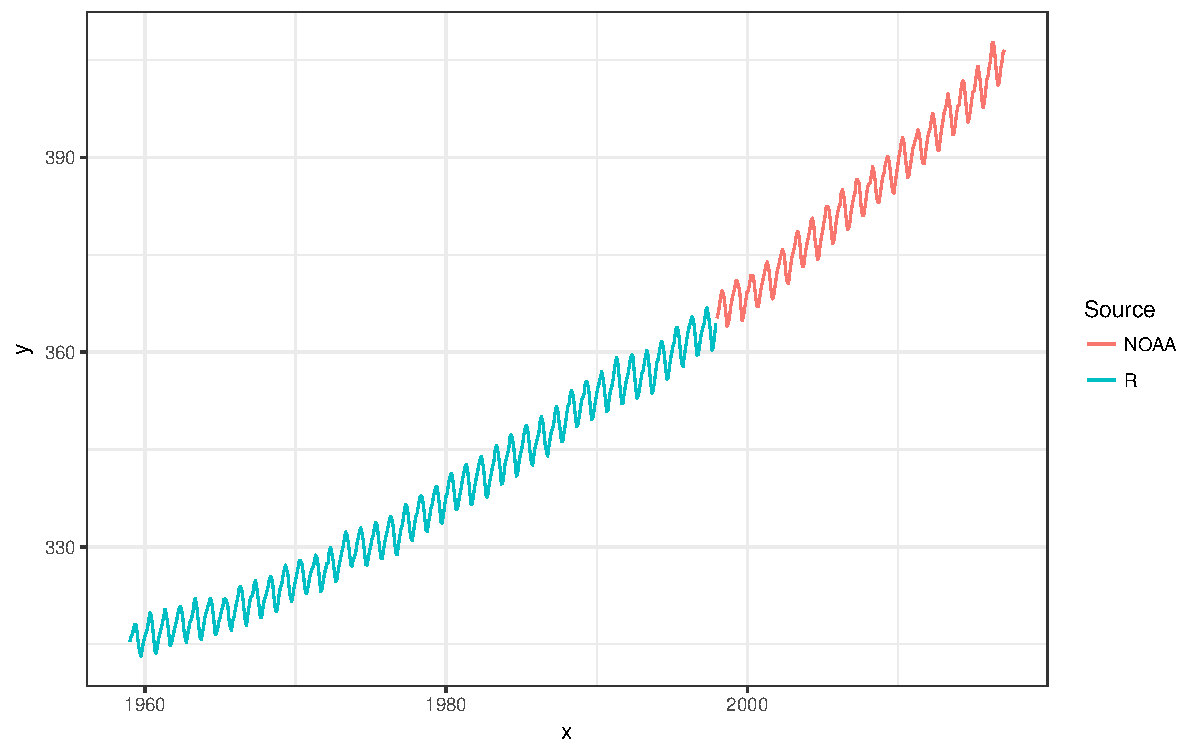
\includegraphics{Lec15_files/figure-beamer/unnamed-chunk-1-1.pdf}

\end{frame}

\begin{frame}{ARIMA}

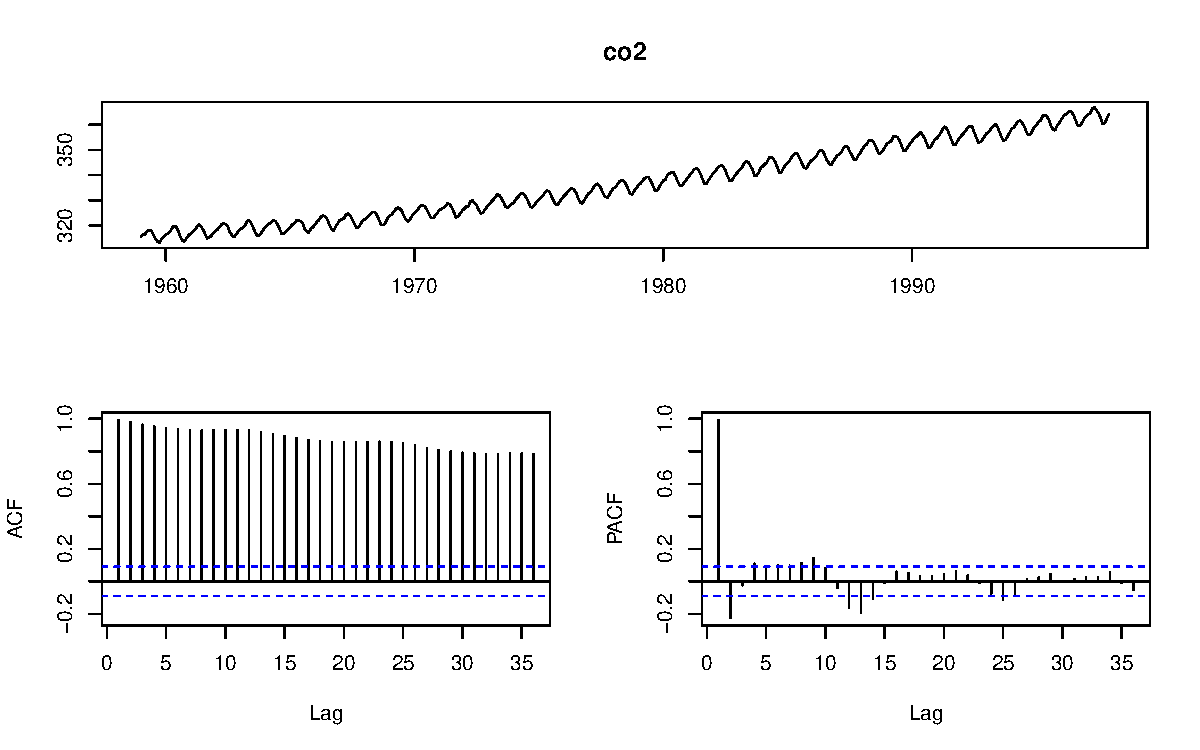
\includegraphics{Lec15_files/figure-beamer/unnamed-chunk-2-1.pdf}

\end{frame}

\begin{frame}[fragile]{ARIMA(0,1,0)\(\times\)(0,0,0)}

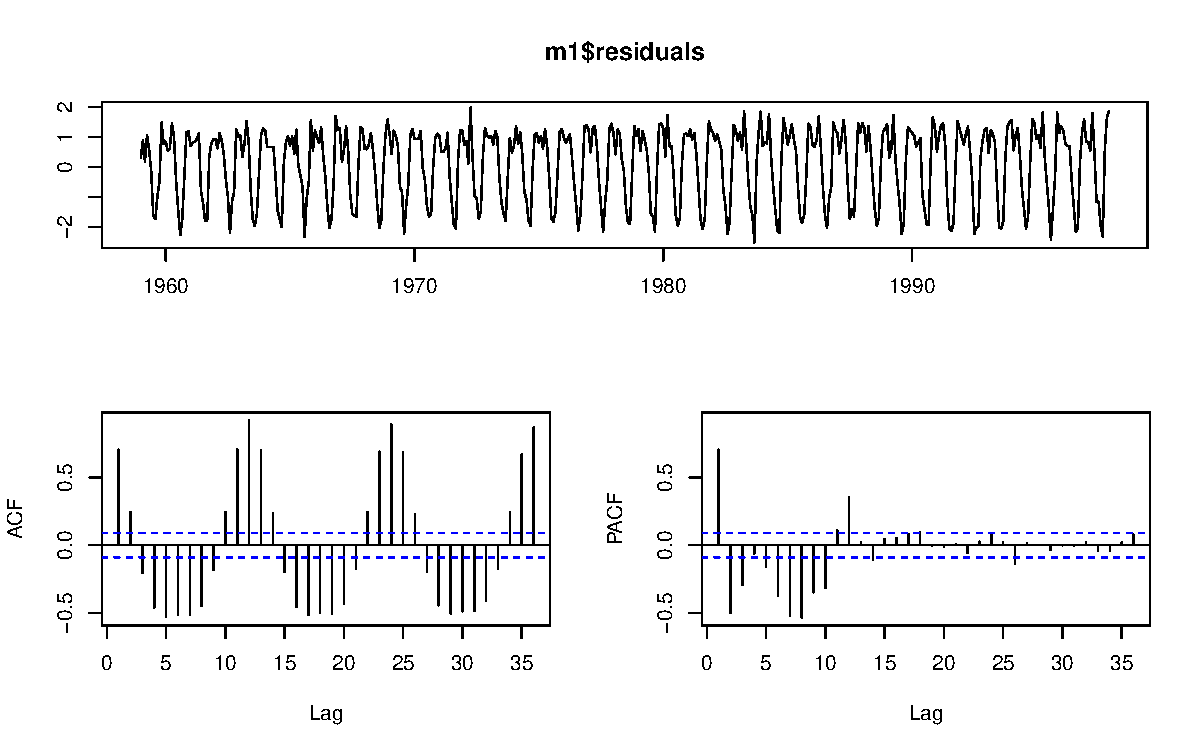
\includegraphics{Lec15_files/figure-beamer/unnamed-chunk-3-1.pdf}

\begin{verbatim}
## [1] 1505.115
\end{verbatim}

\end{frame}

\begin{frame}[fragile]{ARIMA(0,1,0)\(\times\)(0,1,0)\(_{12}\)}

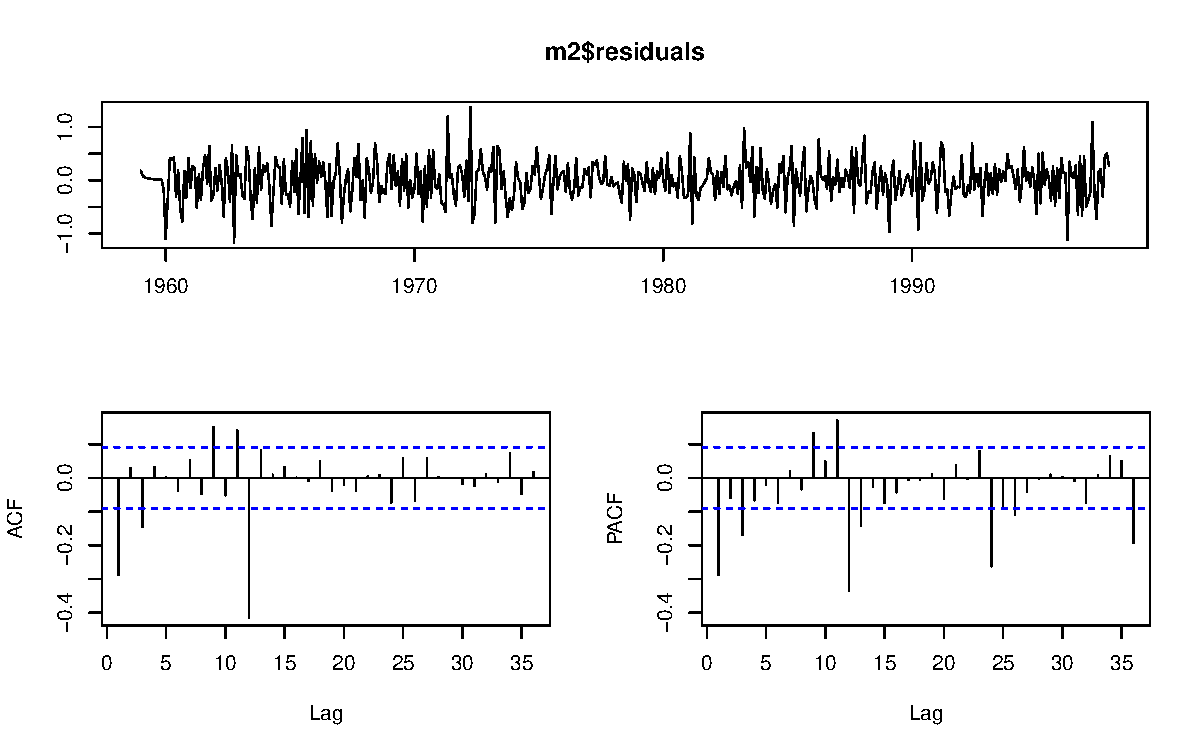
\includegraphics{Lec15_files/figure-beamer/unnamed-chunk-4-1.pdf}

\begin{verbatim}
## [1] 442.0075
\end{verbatim}

\end{frame}

\begin{frame}[fragile]{ARIMA(0,1,0)\(\times\)(0,1,1)\(_{12}\)}

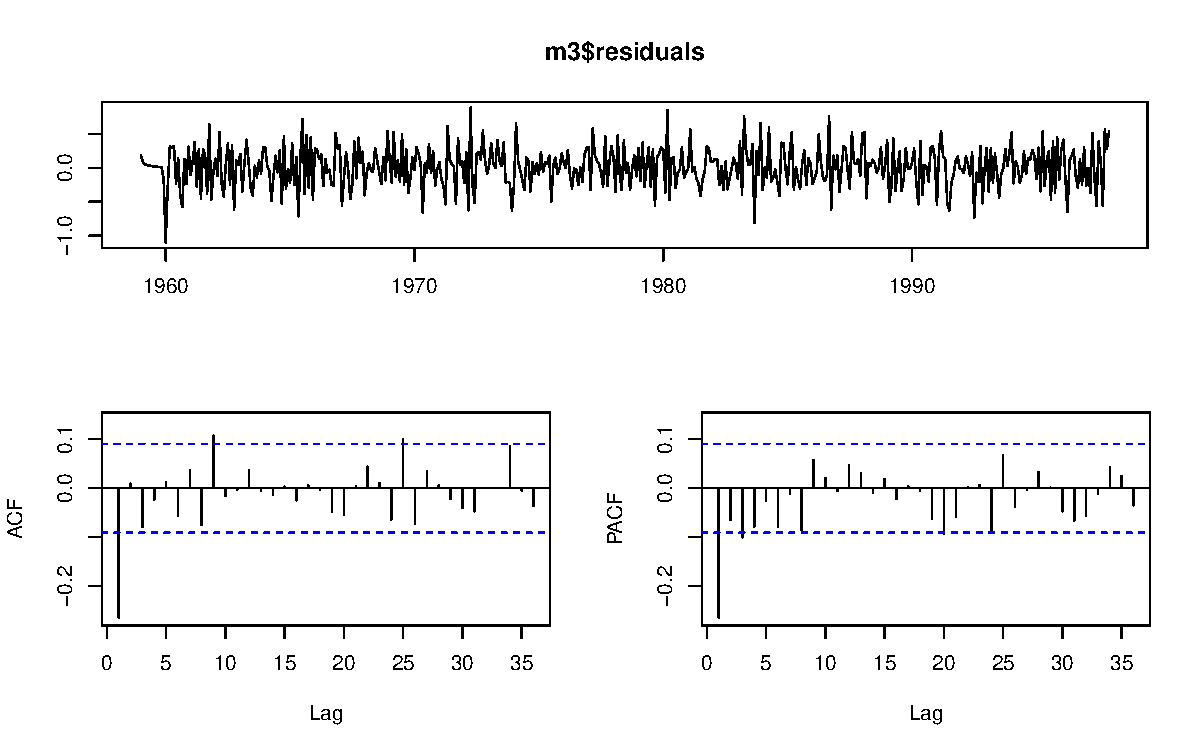
\includegraphics{Lec15_files/figure-beamer/unnamed-chunk-5-1.pdf}

\begin{verbatim}
## [1] 221.5212
\end{verbatim}

\end{frame}

\begin{frame}[fragile]{ARIMA(0,1,1)\(\times\)(0,1,1)\(_{12}\)}

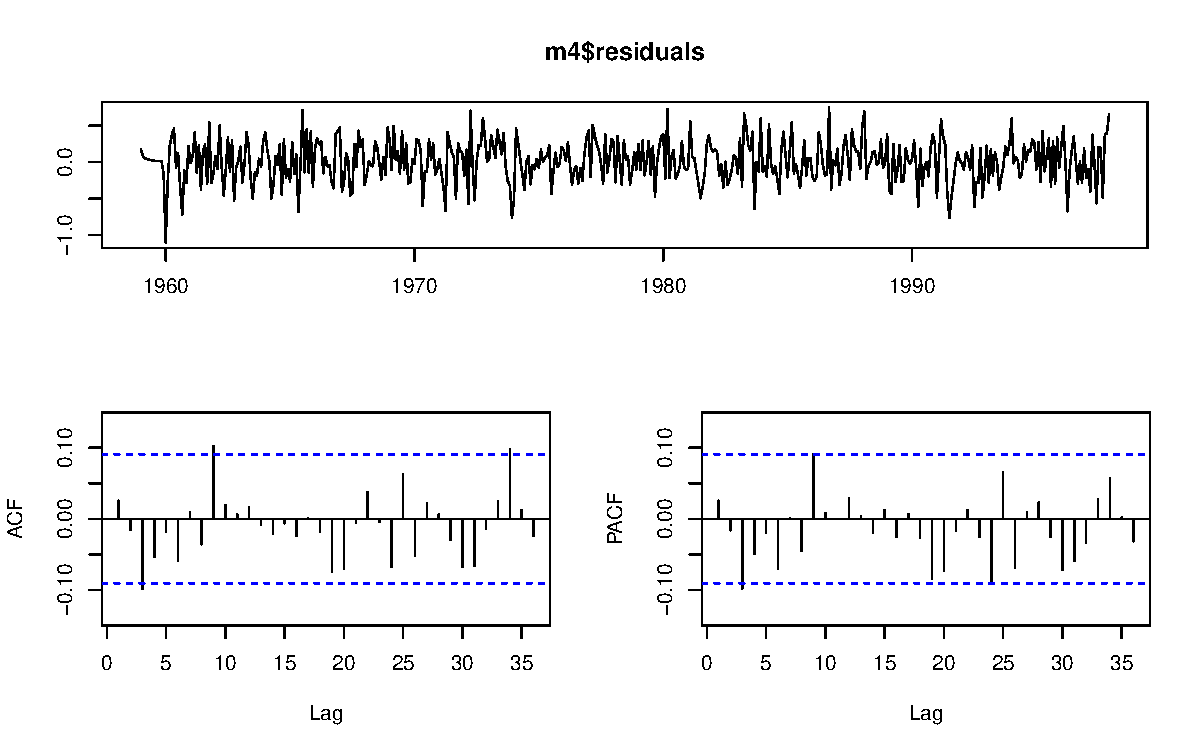
\includegraphics{Lec15_files/figure-beamer/unnamed-chunk-6-1.pdf}

\begin{verbatim}
## [1] 178.2089
\end{verbatim}

\end{frame}

\begin{frame}[fragile]{ARIMA(0,1,3)\(\times\)(0,1,1)\(_{12}\)}

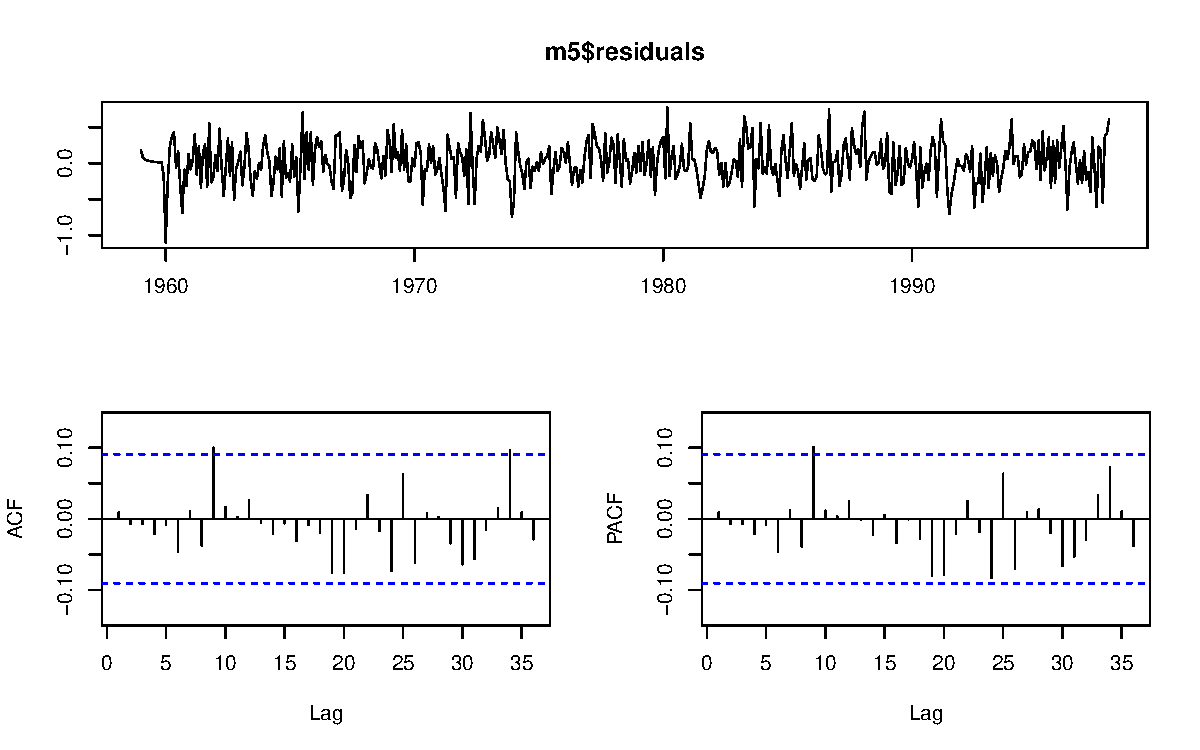
\includegraphics{Lec15_files/figure-beamer/unnamed-chunk-7-1.pdf}

\begin{verbatim}
## [1] 176.9982
\end{verbatim}

\end{frame}

\begin{frame}[fragile]{auto.arima}

\begin{Shaded}
\begin{Highlighting}[]
\KeywordTok{auto.arima}\NormalTok{(co2)}
\NormalTok{## Series: co2 }
\NormalTok{## ARIMA(1,1,1)(1,1,2)[12]                    }
\NormalTok{## }
\NormalTok{## Coefficients:}
\NormalTok{##          ar1      ma1     sar1     sma1     sma2}
\NormalTok{##       0.2569  -0.5847  -0.5489  -0.2620  -0.5123}
\NormalTok{## s.e.  0.1406   0.1203   0.5881   0.5703   0.4820}
\NormalTok{## }
\NormalTok{## sigma^2 estimated as 0.08576:  log likelihood=-84.39}
\NormalTok{## AIC=180.78   AICc=180.97   BIC=205.5}
\end{Highlighting}
\end{Shaded}

\end{frame}

\begin{frame}{Forecasting}

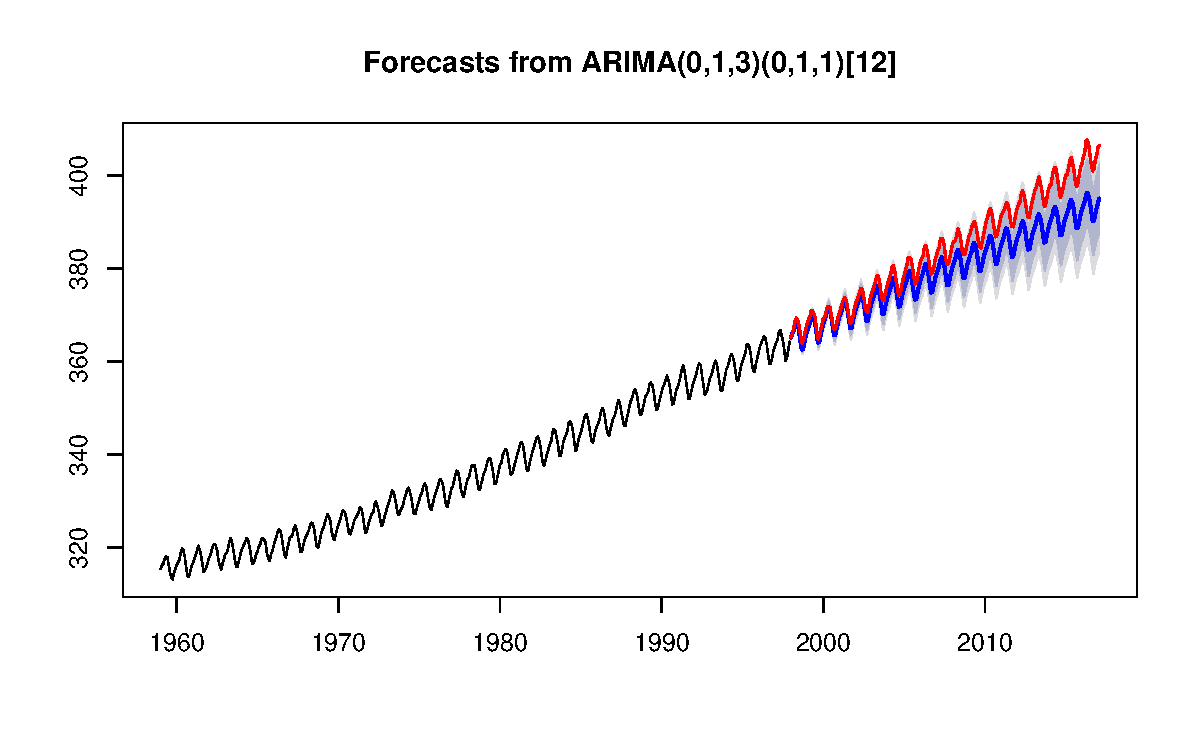
\includegraphics{Lec15_files/figure-beamer/unnamed-chunk-9-1.pdf}

\end{frame}

\begin{frame}{Forecasting (zoom)}

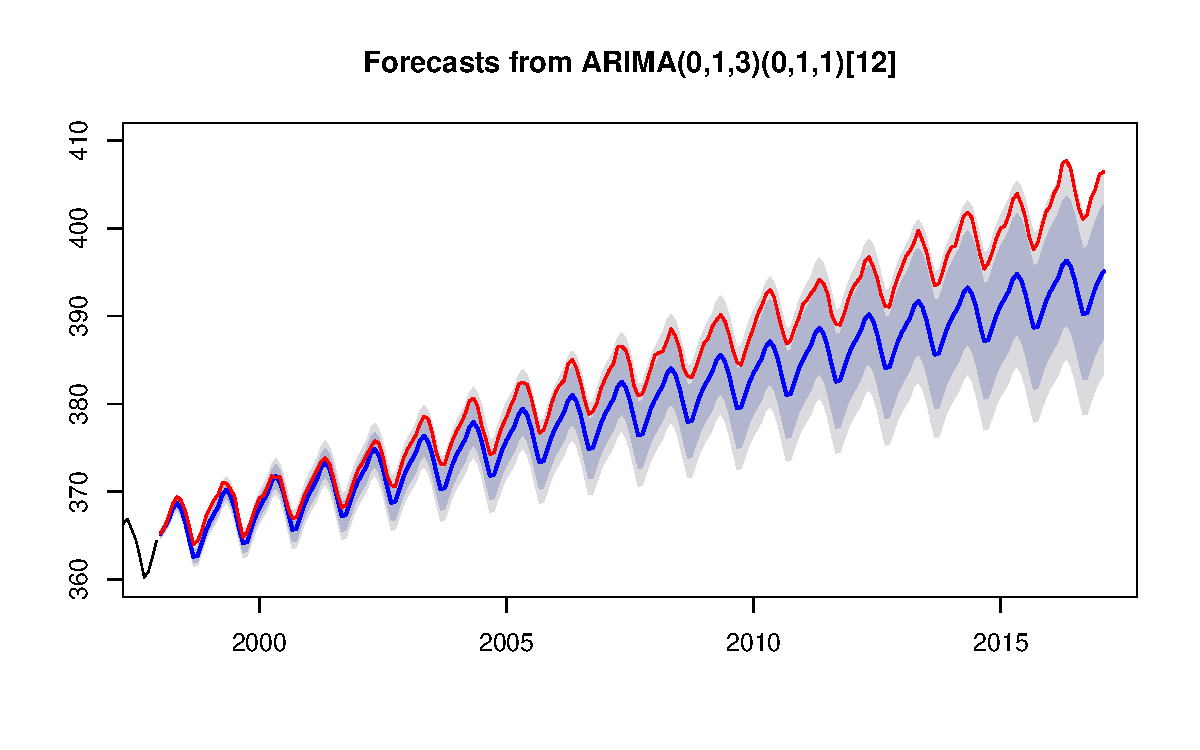
\includegraphics{Lec15_files/figure-beamer/unnamed-chunk-10-1.pdf}

\end{frame}

\begin{frame}[t]{GP Model}

Based on Rasmussen 5.4.3 (we are using slightly different data and
parameterization)

\[ y \sim \mathcal{N}(\bm\mu,~ \bm\Sigma_1 + \bm\Sigma_2 + \bm\Sigma_3 + \bm\Sigma_4 + \sigma^2_5 \mathit{I}\,) \]

\[\{\bm\mu\}_i = \bar{y}\]

\[
\begin{aligned}
\{\bm\Sigma_1\}_{ij} &= \sigma^2_1 \exp\left(-(l_1 \cdot d_{ij})^2\right) \\
\{\bm\Sigma_2\}_{ij} &= \sigma^2_2 \exp\left(-(l_2 \cdot d_{ij})^2\right)\exp\left(-2 \, (l_3)^2  \sin^2(\pi \, d_{ij} / p)\right) \\
\{\bm\Sigma_3\}_{ij} &= \sigma^2_3 \left(1+\frac{(l_4 \cdot d_{ij})^2}{\alpha}\right)^{-\alpha} \\
\{\bm\Sigma_4\}_{ij} &= \sigma^2_4 \exp\left(-(l_5 \cdot d_{ij})^2\right)
\end{aligned}
\]

\end{frame}

\begin{frame}[fragile]{JAGS Model}

\scriptoutput

\begin{verbatim}
## model{
##   y ~ dmnorm(mu, inverse(Sigma))
## 
##   for (i in 1:(length(y)-1)) {
##     for (j in (i+1):length(y)) {
##       k1[i,j] <- sigma2[1] * exp(- pow(l[1] * d[i,j],2))
##       k2[i,j] <- sigma2[2] * exp(- pow(l[2] * d[i,j],2) - 2 * pow(l[3] * sin(pi*d[i,j] / per), 2))
##       k3[i,j] <- sigma2[3] * pow(1+pow(l[4] * d[i,j],2)/alpha, -alpha)
##       k4[i,j] <- sigma2[4] * exp(- pow(l[5] * d[i,j],2))
##       
##       Sigma[i,j] <- k1[i,j] + k2[i,j] + k3[i,j] + k4[i,j]
##       Sigma[j,i] <- Sigma[i,j]
##     }
##   }
## 
##   for (i in 1:length(y)) {
##     Sigma[i,i] <- sigma2[1] + sigma2[2] + sigma2[3] + sigma2[4] + sigma2[5]
##   }  
## 
##   for(i in 1:5){
##     sigma2[i] ~ dt(0, 2.5, 1) T(0,)
##     l[i] ~ dt(0, 2.5, 1) T(0,)
##   }
##   alpha ~ dt(0, 2.5, 1) T(0,)
## }
\end{verbatim}

\end{frame}

\begin{frame}{Forecasting}

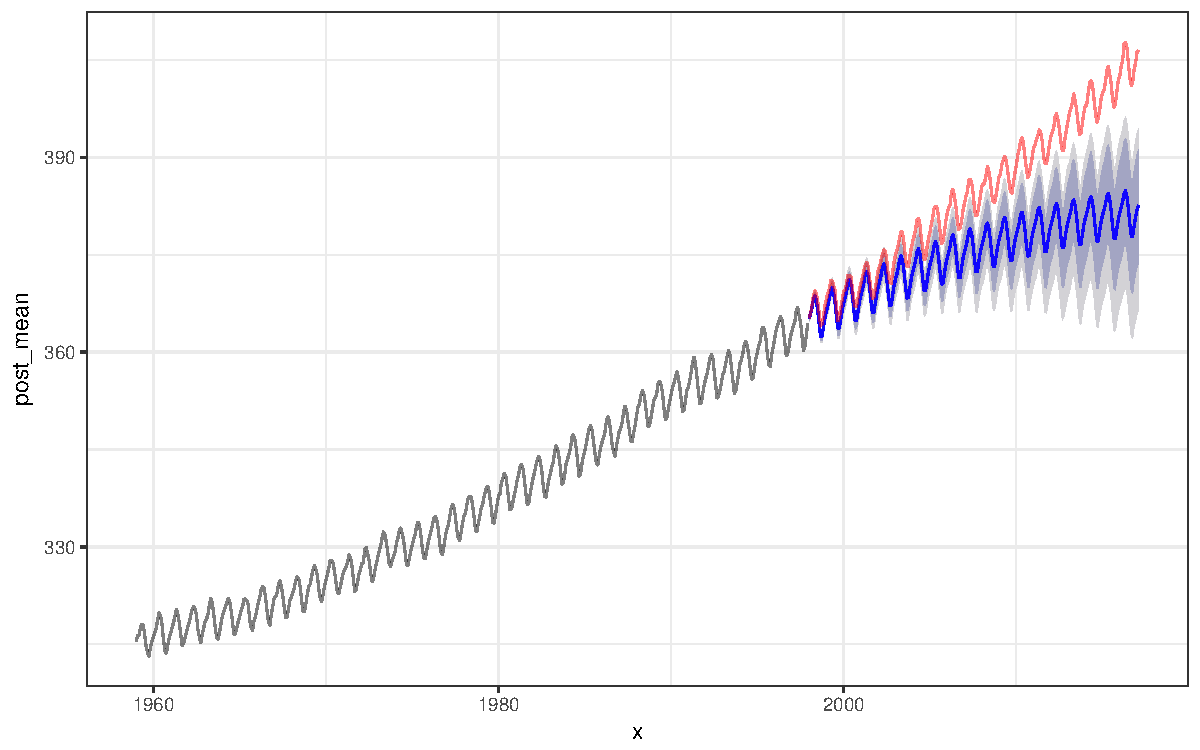
\includegraphics{Lec15_files/figure-beamer/unnamed-chunk-16-1.pdf}

\end{frame}

\begin{frame}{Forecasting (zoom)}

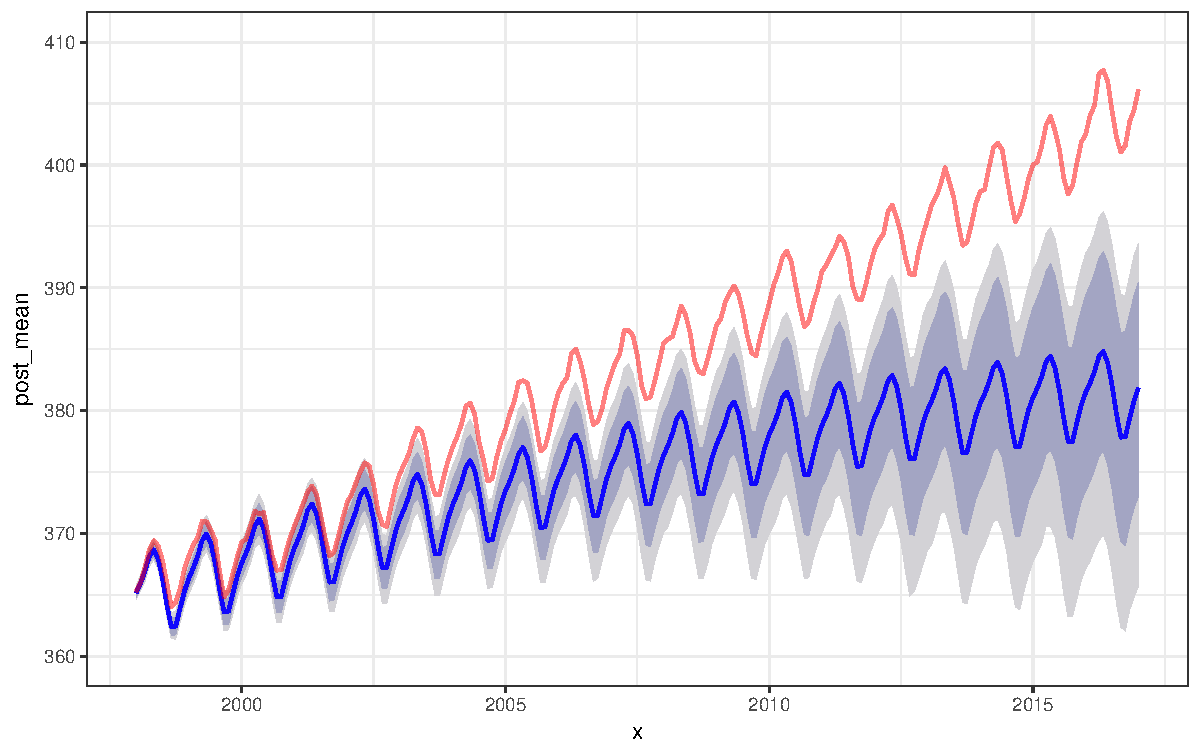
\includegraphics{Lec15_files/figure-beamer/unnamed-chunk-17-1.pdf}

\end{frame}

\begin{frame}{Forecasting RMSE}

\begin{longtable}[]{@{}lrr@{}}
\toprule
dates & RMSE (arima) & RMSE (gp)\tabularnewline
\midrule
\endhead
Jan 1998 - Jan 2003 & 1.119 & 1.911\tabularnewline
Jan 1998 - Jan 2008 & 2.521 & 4.575\tabularnewline
Jan 1998 - Jan 2013 & 3.839 & 7.706\tabularnewline
Jan 1998 - Mar 2017 & 5.474 & 11.395\tabularnewline
\bottomrule
\end{longtable}

\end{frame}

\begin{frame}[t]{Rewriting the GP likelihood}

From last time, remember that we can view our GP in the following ways,

\[ y \sim \mathcal{N}(\bm\mu,~ \bm\Sigma_1 + \bm\Sigma_2 + \bm\Sigma_3 + \bm\Sigma_4 + \sigma^2_5 \mathit{I}\,) \]

but we can also think of \(y\) as being the deterministic sum of 5
independent GPs

\[ y = \mu + w_1(\bm{x}) + w_2(\bm{x}) + w_3(\bm{x}) + w_4(\bm{x}) + w_5(\bm{x}) \]
where \[
\begin{aligned}
w_1(\bm{x}) &\sim \mathcal{N}(0, \bm\Sigma_1) \\
w_2(\bm{x}) &\sim \mathcal{N}(0, \bm\Sigma_2) \\
w_3(\bm{x}) &\sim \mathcal{N}(0, \bm\Sigma_3) \\
w_4(\bm{x}) &\sim \mathcal{N}(0, \bm\Sigma_4) \\
w_5(\bm{x}) &\sim \mathcal{N}(0, \sigma^2_5 \mathit{I}\,)
\end{aligned}
\]

\end{frame}

\begin{frame}[t]{Decomposition of Covariance Components}

\footnotesize
\[ \begin{bmatrix} 
w_1(\bm{x}) \\
w_1(\bm{x}^\star) \\
w_2(\bm{x}) \\
\bm{y}
\end{bmatrix} 
\sim \mathcal{N} \left(
\begin{bmatrix}
0 \\ 0\\ 0\\ \bm{\mu}
\end{bmatrix},~
\begin{bmatrix}
\Sigma_1 & \Sigma_1^\star & 0 & \Sigma_1 \\
{\Sigma_1^\star}^t & \Sigma_1^{\star\star} & 0 & \Sigma_1^\star \\
0 & 0 & \Sigma_2 & \Sigma_2 \\
\Sigma_1 & \Sigma_1^\star & \Sigma_2 & \sum_{i=1}^5 \Sigma_i
\end{bmatrix}
\right)
\]

\normalsize

therefore

\[ w_1(\bm{x}^\star) ~|~ \bm{y},\bm\mu,\bm\theta \sim \mathcal{N}(\mu_{cond},~ \Sigma_{cond}) \]

\[ \mu_{cond} = 0 + \Sigma_1^\star (\Sigma_1 + \Sigma_2 + \Sigma_3 + \Sigma_4 + \Sigma_5)^{-1}(\bm{y}-\bm\mu) \]
\[ \Sigma_{cond} = \Sigma_1^{\star\star} - \Sigma_1^\star (\Sigma_1 + \Sigma_2 + \Sigma_3 + \Sigma_4 + \Sigma_5)^{-1} {\Sigma_1^\star}^t \]

\end{frame}

\begin{frame}{Forecasting Components}

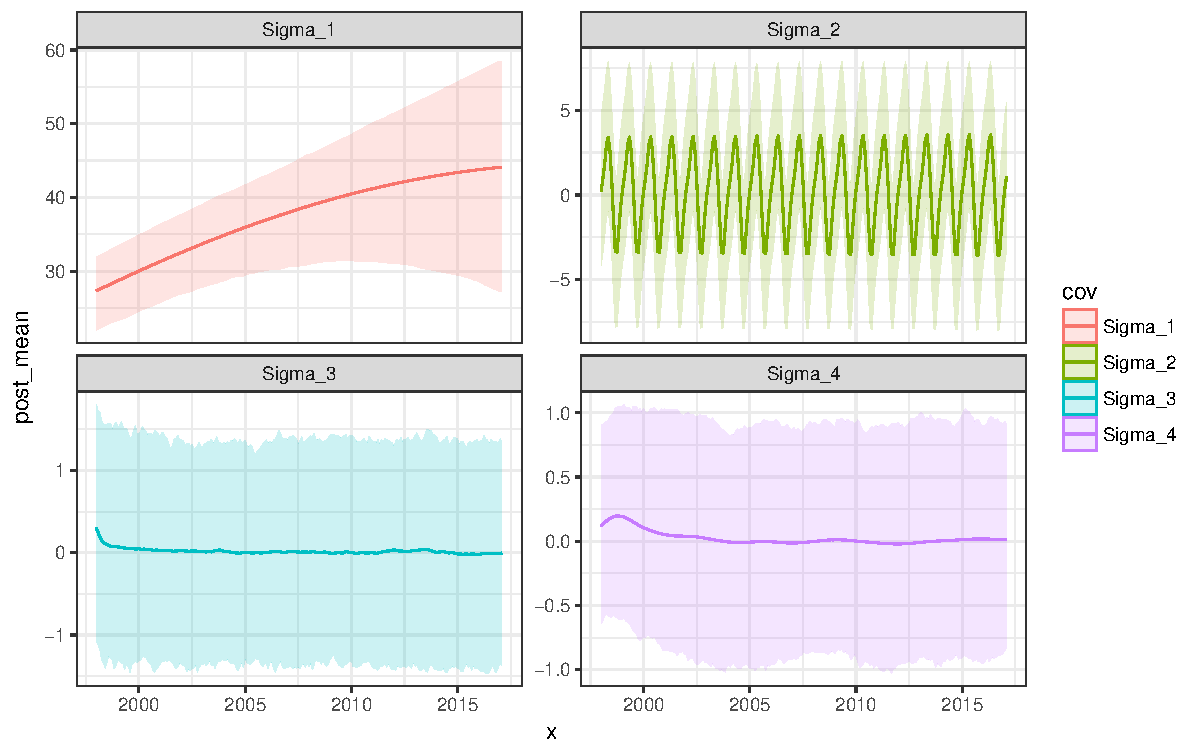
\includegraphics{Lec15_files/figure-beamer/unnamed-chunk-20-1.pdf}

\end{frame}

\begin{frame}{Fit Components}

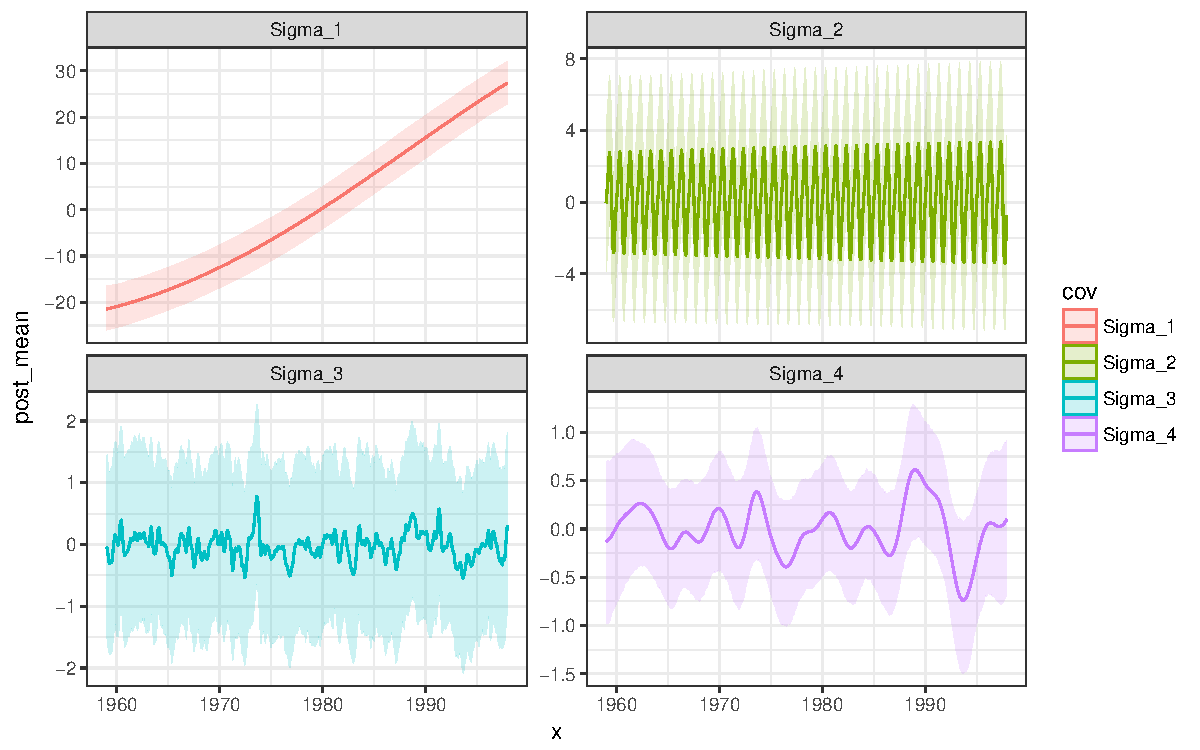
\includegraphics{Lec15_files/figure-beamer/unnamed-chunk-22-1.pdf}

\end{frame}

\section{GPs and Logistic Regression}\label{gps-and-logistic-regression}

\begin{frame}[t]{Logistic Regression}

A typical logistic regression problem uses the following model,

\[y_i \sim \text{Bern}(p_i)\] \[\begin{aligned}
\text{logit}(p_i) 
  &= \bm{X}\,\bm{\beta} \\
  &= \beta_0 + \beta_1 \, x_{i1} + \cdots + \beta_k \, x_{ik}
\end{aligned}\]

\pause

there is no reason that the linear equation above can't contain thing
like random effects or GPs

\[\begin{aligned}
y_i &\sim \text{Bern}(p_i) \\
\text{logit}(p_i) 
  &= \bm{X}\,\bm{\beta} + w(\bm{x}) \\
\end{aligned}\] where \[ w(\bm{x}) \sim \mathcal{N}(0,\Sigma)\]

\end{frame}

\begin{frame}{A toy example}

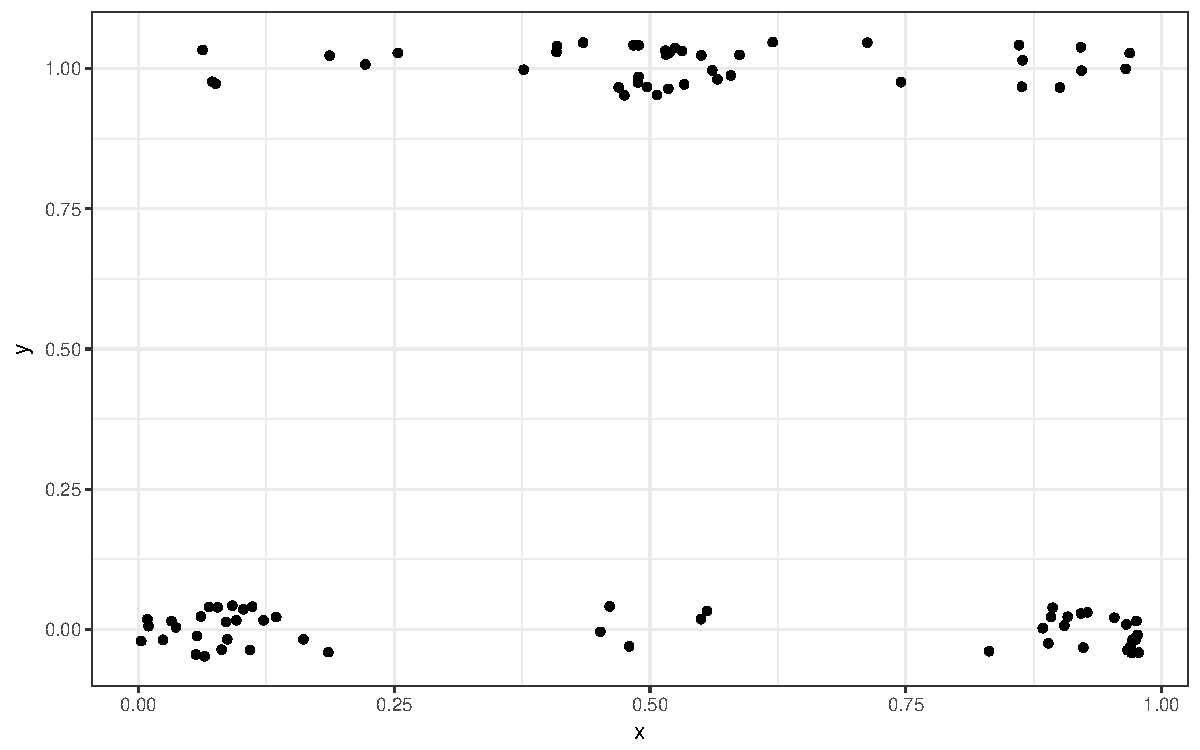
\includegraphics{Lec15_files/figure-beamer/unnamed-chunk-23-1.pdf}

\end{frame}

\begin{frame}[fragile]{Jags Model}

\footnoteoutput

\begin{verbatim}
## model{
##   for(i in 1:N) {
##     y[i] ~ dbern(p[i])
##     logit(p[i]) <- eta[i]
##   }
##   eta ~ dmnorm(rep(0,N), inverse(Sigma))
## 
##   for (i in 1:(length(y)-1)) {
##     for (j in (i+1):length(y)) {
##       Sigma[i,j] <- sigma2 * exp(- pow(l * d[i,j],2))
##       Sigma[j,i] <- Sigma[i,j]
##     }
##   }
## 
##   for (i in 1:length(y)) {
##     Sigma[i,i] <- sigma2 + 1e-06
##   }  
## 
##   sigma2 ~ dt(0, 2.5, 1) T(0,)
##   l ~ dunif(sqrt(3),100)
## }
\end{verbatim}

\end{frame}

\end{document}
